\section{Pengujian \& Evaluasi}

\subsection{Kecepatan Sistem}
Pengujian kecepatan dilakukan dengan menggunakan Google Chrome Developer Tools, dimana untuk setiap kasus penggunaan diuji dengan segmentasi \textit{loading time} sebagai berikut \begin{inlinelist}
	\item \textit{DOM Loading}
	\item \textit{Scripting}
	\item \textit{Rendering}
\end{inlinelist}. Rata-rata keseluruhan \textit{loading page} adalah 3,2 detik (lebih 6\% dari target). Untuk menganalisa dengan visualisasi masing-masing segmen pada Gambar \ref{bar-chart-speed}.
\begin{figure}[h!]
	\centering
	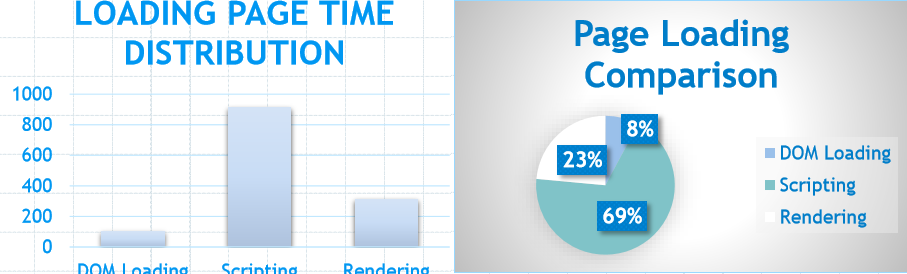
\includegraphics[width=.45\textwidth]{images/bab5/speed/combined.png}
	\caption{Diagram Visualisasi dan Perbandingan Waktu per Segmen}
	\label{bar-chart-speed}
\end{figure}
	Dengan menggunakan \textit{tool} Lighthouse, \textit{scripting} memakan waktu yang sangat besar (hampir 75|\% \textit{loading time}) untuk \textit{loading} gambar, yang ternyata ini menjadi masalah umum pada website \textit{e-commerce}, dimana penyelesaiannya menggunakan teknik \textit{image optimization}.

\subsection{\textit{Maintainability Assesment}}
Pengujian \textit{maintainability} dilakukan dengan mengikuti pedoman dari paper "A Software Maintainability Evaluation Methodology"\cite{peercy_software_nodate}, yaitu parameter utama: \textit{modularity},\textit{descriptiveness},\textit{consistency},\textit{simplicity}, dan \textit{trackability}.Sesuai dengan paper tersebut, dengan dua aspek penilaian - kode sumber dan dokumentasi sistem dengan \textit{weight} masing-masing yang berbeda - rekapitulasi hasil dapat dilihat pada Gambar \ref{maintainability-recap}, dan visualisasi dalam bentuk diagram dapat dilihat pada Gambar \ref{maintainability-chart}.
\begin{figure}[h!]
	\centering
	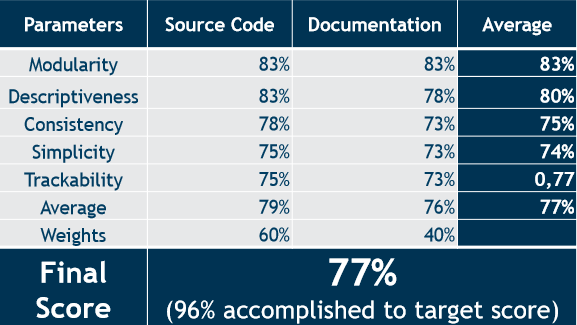
\includegraphics[width=.45\textwidth]{images/bab5/maintainability/telor.png}
	\caption{Diagram Perbandingan Hasil per Parameter pada \textit{Maintainability Assesment}}
	\label{maintainability-recap}
\end{figure}
\begin{figure}[h!]
	\centering
	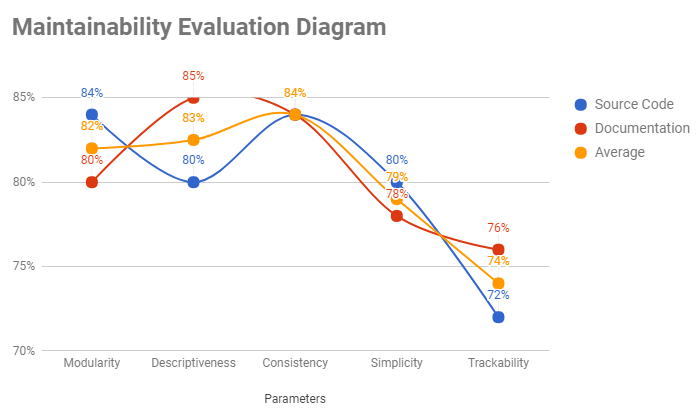
\includegraphics[width=.45\textwidth]{images/bab5/maintainability/maintainability-evaluation.png}
	\caption{Diagram Perbandingan Hasil per Parameter pada \textit{Maintainability Assesment}}
	\label{maintainability-chart}
\end{figure}
\subsection{\textit{User Experience Assesment}}
Pengujian \textit{maintainability} dilakukan dengan mengikuti pedoman dari paper " Development of an Instrument Measuring User Satisfaction of the Human-Computer Interface"\cite{chin_development_1998}. Rekapitulasi hasil dapat dilihat pada Gambar \ref{ux-recap}, dan visualisasi hasil berbentuk diagram dapat dilihat pada Gambar \ref{ux-chart}.
\begin{figure}[h!]
	\centering
	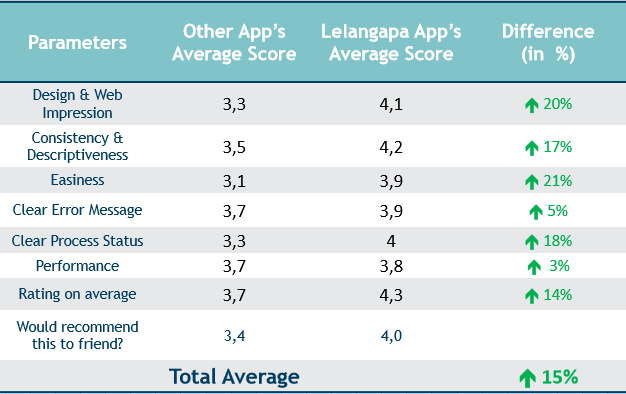
\includegraphics[width=.45\textwidth]{images/bab5/ujipengguna/result.png}
	\caption{Rekapitulasi Hasil \textit{User Experience Assesment}}
	\label{ux-recap}
\end{figure}
\begin{figure}[h!]
	\centering
	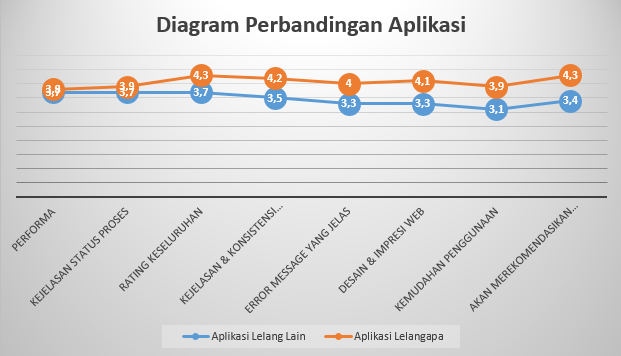
\includegraphics[width=.45\textwidth]{images/bab5/ujipengguna/chart.png}
	\caption{Visualisasi Perbandingan Hasil \textit{User Experience Assesment} Aplikasi dengan Aplikasi Lainnya}
	\label{ux-chart}
\end{figure}